\section{Relationen}
\begin{def*}[note = Relation , index = Relation]
	Eine (binäre) Relation $\mathrm{R}$ von $A$ nach $B$ ist $\mathrm{R} \subseteq A \times B$ . \\
	Relation auf $A$: $\mathrm{R} \subseteq A \times A = A^2$
\end{def*}
\[
	\text{Wir schreiben } \begin{array}{ l l l }
		a &\mathrm{R}		&b			\\
		a &\leq			&b			\\
		a &\not{\mathrm{R}}	&b			\\
		a &\not\leq		&b	
	\end{array} \text{ für } \begin{array}{ l l l }
		(a , b) &\in			&\mathrm{R}	\\
		(a , b) &\in			&\leq			\\
		(a , b) &\notin		&\mathrm{R}	\\
		(a , b) &\notin		&\leq		
	\end{array}
\]
Jetzt sind die Relationen Mengen $\rightarrow$ Mengenkalkül
\begin{gather*}
	\leq~\cap~\geq~=~= \\
	\leq~\bigtriangleup~\geq~=~\neq \\
	<~\subseteq~\leq~=~\overline{\geq}~=~\leq
\end{gather*}
\begin{bsp*}{Relationen auf $\Z$}
	$\mathrm{R} \subset \mathbb{Z} \times \mathbb{Z}$ \\
	\begin{itemize}
		\item $\mid$ Teilbarkeit: \quad $(a , b) \in \mid :\iff \exists c \in \mathbb{Z} : a \cdot c = b$
		\item $\leq$
		\item $\equiv \pmod m \quad a \equiv b \pmod m :\iff m \mid (a - b)$ \\
			$ \equiv_m \cap \equiv_n = \equiv_{kgV(m,n)}$
	\end{itemize}
\end{bsp*}

\subsubsection{Darstellung von Relationen}
falls $|A| , |B| < \infty$\\
Relation $\mathrm{R}$ von $A$ nach $B , \mathrm{R} \subseteq A \times B$\\
\begin{description}
	\item[Als (binäre) Matrix] Eintrag ist $1$ falls $(a , b) \in \mathrm{R}$, sonst $0$
	\item[Als bipartiter Graph] 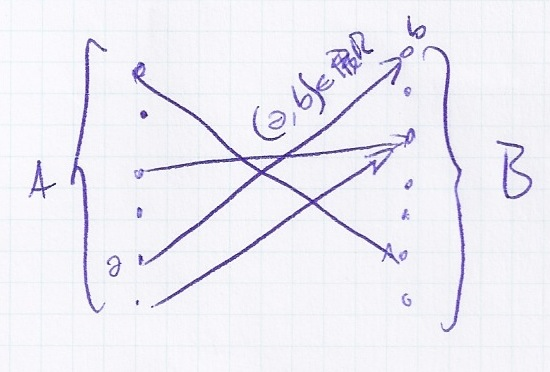
\includegraphics{Bild15}
	\item[Falls $A = B$] 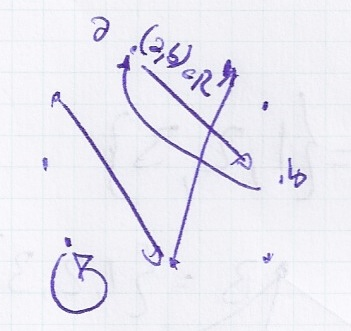
\includegraphics{Bild16}
\end{description}

\subsubsection{Eigenschaften von Relationen (auf \texorpdfstring{$A$}{A})}
\begin{description}
	\item[reflexiv:] $\forall a \in A : (a , a) \in \mathrm{R}$
		\begin{itemize}
			\item Matrix: Diagonale lauter 1 \\
				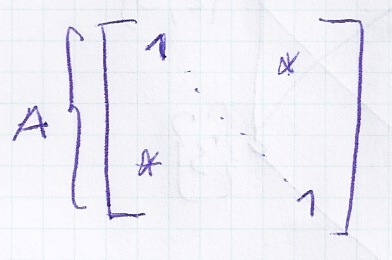
\includegraphics{Bild17}
			\item Graph: jede Punkt mit sich selbst (loop) \\
				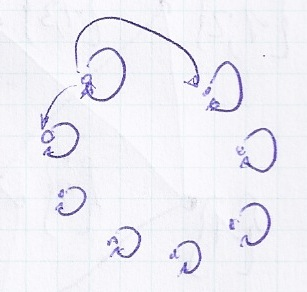
\includegraphics{Bild18} \\
			\begin{bsp*}{reflexive Relationen}\\
				\begin{itemize}
					\item $\leq$
					\item $=$
					\item $|$
					\item $\subseteq$
					\item $\equiv_m$
				\end{itemize}
			\end{bsp*}
			\begin{bsp*}{nicht reflexive Relationen}
				\begin{itemize}
					\item $<$
					\item $>$
					\item $\subset$
					\item $\nmid$
					\item $\neq$
					\item $\in$
				\end{itemize}
			\end{bsp*}
		\end{itemize}
	\item[antireflexiv:] $\forall a \in A : (a , a) \notin \mathrm{R}$
		\begin{itemize}
			\item Matrix: Diagonale lauter $0$
			\item Graph: Kein Punkt mit sich selbst
		\end{itemize}
	\item[symmetrisch:] $\forall a , b \in A : (a , b) \in \mathrm{R} \iff (b , a) \in \mathrm{R}$
		\begin{itemize}
			\item Matrix: symmetrisch $(M^T = M)$
			\item Graph: alle Pfeile beidseitig (werden als Linien ohne Pfeilköpfe dargestellt) \\
			\begin{bsp*}{symmetrische Relationen}
				\begin{itemize}
					\item $=$
					\item $\equiv_m$
				\end{itemize}
			\end{bsp*}
		\end{itemize}
	\item[antisymmetrisch:] $\forall a , b \in A : (a , b) \in \mathrm{R} \wedge (b , a) \in \mathrm{R} \implies a = b$\\
		\begin{bsp*}{antisymmetrische Relationen}
			\begin{itemize}
				\item $\leq$
				\item $|$ auf $\mathbb{N}$
				\item $<$
				\item $=$
			\end{itemize}
		\end{bsp*}
	\item[transitiv:] $\forall a , b , c \in A : (a , b) \in \mathrm{R} \wedge (b , c) \in \mathrm{R} \implies (a , b) \in \mathrm{R}$\\
		\begin{itemize}
			\item Graph: Pfeilkette $\implies$ direkter Pfeil \\
			\begin{bsp*}[note = transitive Relationen]
				\begin{itemize}
					\item $\leq$
					\item$>$
					\item $=$
					\item $\equiv_m$
					\item $|$
					\item $\subseteq$
				\end{itemize}
			\end{bsp*}
			\begin{bsp*}[note = nicht transitive Relationen]
				\begin{itemize}
					\item $\neq$
					\item $\not\leq$
					\item $\not\equiv_m$
					\item $\in$ denn: \\
						\begin{gather*}
							\varnothing \in \{ \varnothing \} \in \{ \{ \varnothing \} \} \\
							\varnothing \notin \{ \{ \varnothing \} \}
						\end{gather*}
				\end{itemize}
			\end{bsp*}
		\end{itemize}
\end{description}

\subsubsection{Transitiver Abschluss \texorpdfstring{$\mathrm{R}'$}{R'} von \texorpdfstring{$\mathrm{R}$}{R}}
$(a , b) \in \mathrm{R}' :\iff \exists c_1 , c_2 , \dotsc , c_n : (a , c_1) \in \mathrm{R} \wedge (c_1 , c_2) \in \mathrm{R} \wedge \dotsb \wedge (c_{n-1} , c_n) \in \mathrm{R} \wedge (c_n , b) \in \mathrm{R}$ \\
Eigenschaften:\\
\begin{itemize}
	\item $\mathrm{R}' \supseteq \mathrm{R}$
	\item $\mathrm{R}'$ transitiv
	\item $\forall S : S \supseteq R , S \text{ transitiv}, S \supseteq \mathrm{R}'$
\end{itemize}
